\documentclass[10pt]{article}

\usepackage{fullpage}
\usepackage{microtype}
\usepackage[english]{babel}
\usepackage[en-GB]{datetime2}
\usepackage[margin=3.5cm]{geometry}
\usepackage{graphicx}
\usepackage{biblatex}
\addbibresource{bibliography.bib}
\parindent=0pt
\frenchspacing
\raggedright

%%For formatting code, usage: \lstinputlisting{iets.cc}
%\usepackage{listings}
%\lstset{language=C++, showstringspaces=false, basicstyle=\small,
%  numbers=left, numberstyle=\tiny, numberfirstline=false,
%  breaklines=true,
%  stepnumber=1, tabsize=8,
%  commentstyle=\ttfamily, identifierstyle=\ttfamily,
%  stringstyle=\itshape}

\title{MGAIA Assignment 1: Procedural Content Generation}
\date{\today}
\author{Eva van Houten, s1478621}

\begin{document}
\maketitle

\section{Introduction}
For this assignment we are studying procedural content generation. We will be automatically generating a house in Minecraft, using the GDPC Python package \cite{GDPC} and the GDMC (Generative Design in Minecraft Challenge) \cite{GDMC} HTTP interface mod \cite{mod}. This mod was created for a contest where people procedurally generate settlements in Minecraft, in a specified building area. The challenge here, which we will explore in this assignment as well, is to adapt the generated structures to the world that is given to you, while also varying what is generated.

\section{Implementation}
Our implementation consists of two main parts: finding a suitable part of the given build area to build in, and actually constructing the house.
\subsection{Finding a build area}
To find a suitable building area, we have written an algorithm that finds all the continuous, flat planes inside the larger area. To accomplish this, we take the following steps:
\begin{itemize}
    \item Take the heightmap that GDPC generates for us
    \item Sort every coordinate point in this heightmap matrix by height
    \item Within every height category, generate a set of continuous points
          \begin{itemize}
              \item Choose a reference coordinate
              \item Check for each point whether it is a neighbour of the reference point, or previously found neighbours of the reference points
              \item Add the neighbours to the set of continuous points
              \item When there are no more new continuous points, we are done
          \end{itemize}
\end{itemize}

The result can be seen in figures~\ref{fig:heightmap},~\ref{fig:cont_map},~and~\ref{fig:plane_map}. Firstly, figure~\ref{fig:heightmap} shows the height map, generated directly from the terrain by GDPC. Figure~\ref{fig:cont_map} shows the result of our algorithm. The difference with the height map is subtle, as there are many different plains, but we can easily see that there are more colour levels in this plot than in the height map. This means the algorithm has subdivided the height levels into their continuous parts. Finally, figure~\ref{fig:plane_map} shows the largest plane we have found, that is the plane with the largest surface area, in yellow. We will be working with this plane to build our house on.

\begin{figure}
    \includegraphics[width=0.5\textwidth]{../plots/heightmap.png}
    \centering
    \caption{A height map of a piece of Minecraft terrain. The colours represent the block height, as defined by the scale on the right of the figure.}
    \label{fig:heightmap}
\end{figure}
\begin{figure}
    \includegraphics[width=0.5\textwidth]{../plots/cont_map.png}
    \centering
    \caption{The heat map of continuous planes, generated from the height map in figure~\ref{fig:heightmap}. The colour scale here does not have a special meaning, but simply numbers all the planes that were found.}
    \label{fig:cont_map}
\end{figure}
\begin{figure}
    \includegraphics[width=0.5\textwidth]{../plots/plane_map.png}
    \centering
    \caption{The largest plane in figure~\ref{fig:cont_map}, hightlighted in yellow.}
    \label{fig:plane_map}
\end{figure}

\subsection{Construction}
In this section we will describe the construction of the house, with regard to its architectural style, how we addressed believability, and how we executed the actual building.
\subsubsection{Architectural style}

I took my inspiration for the architectural style from the image in figure~\ref{fig:style}. It contains a wooden holiday cabin in Norway. I have implemented this style by constructing a simple cabin with a veranda on two sides. I have chosen the spruce log block for the walls, and the spruce planks for the roof, to match the cabin's wood texture and colours. The roof has an overhang over the veranda, and the door is a light colour to represent the light details in the reference house. %TODO check woods
% TODO reference https://woodmasters.com.ua/wp-content/uploads/2015/01/1392040471-848x480.jpg 20 jun 2023

\begin{figure}
    \includegraphics[width=0.5\textwidth]{style.jpg}
    \centering
    \caption{An example of a Norwegian wood cabin, that I took as inspiration for my Minecraft house.}
    \label{fig:style}
\end{figure}

\subsubsection{Believability}
To address believability, I have implemented the following qualities:
\begin{itemize}
    \item Placement\\
          The house is placed in the largest continuous flat area. This ensures that no features of the landscape need to be changed. This would be a realistic place to build a real house, since minimal digging would be required to prepare the building site. The construction algorithm also takes into account a small margin of one block on every side of the house, such that no wall is placed directly against the slope of a hill.
    \item Size\\
          The house's size is adapted to the amount of space available. The maximum size is 12x10 blocks, since this represents a comfortably large, but not extravagant, cabin. The minimum size is 5x5 blocks for the house itself, to allow room for a door or window on each wall, and 3x3 blocks of indoor space. With the veranda, this comes to 7x7 blocks total.
    \item Facing direction\\
          To determine which sides of the house are equipped with a veranda, we use the\\ \texttt{getOptimalFacingDirection} function that GDPC provides. This function yields a ranked list of best, unobstructed directions for a structure to face. Since the function does not always return two top directions (for the two veranda sides), we augment the result with a basic heuristic: people in cold countries, like the Norwegians, always want to sit facing the south, to catch as much sun and warmth as possible. They also like to sit outside in the evening and catch some sun, so the secondary preference would be to face east.
    \item Window and door placement\\
          The door is always placed on a welcoming veranda side, with a fence gate and stairs leading to it. The door and windows are also always placed with two blocks of wall on either corner, to make the house make sense on the inside. The windows are always placed symmetrically, and the placement of the door is somewhat randomised.
\end{itemize}

\subsubsection{Constructing}
%TODO

\section{Results: variation and adaptability}
Figures with examples:
\begin{figure}
    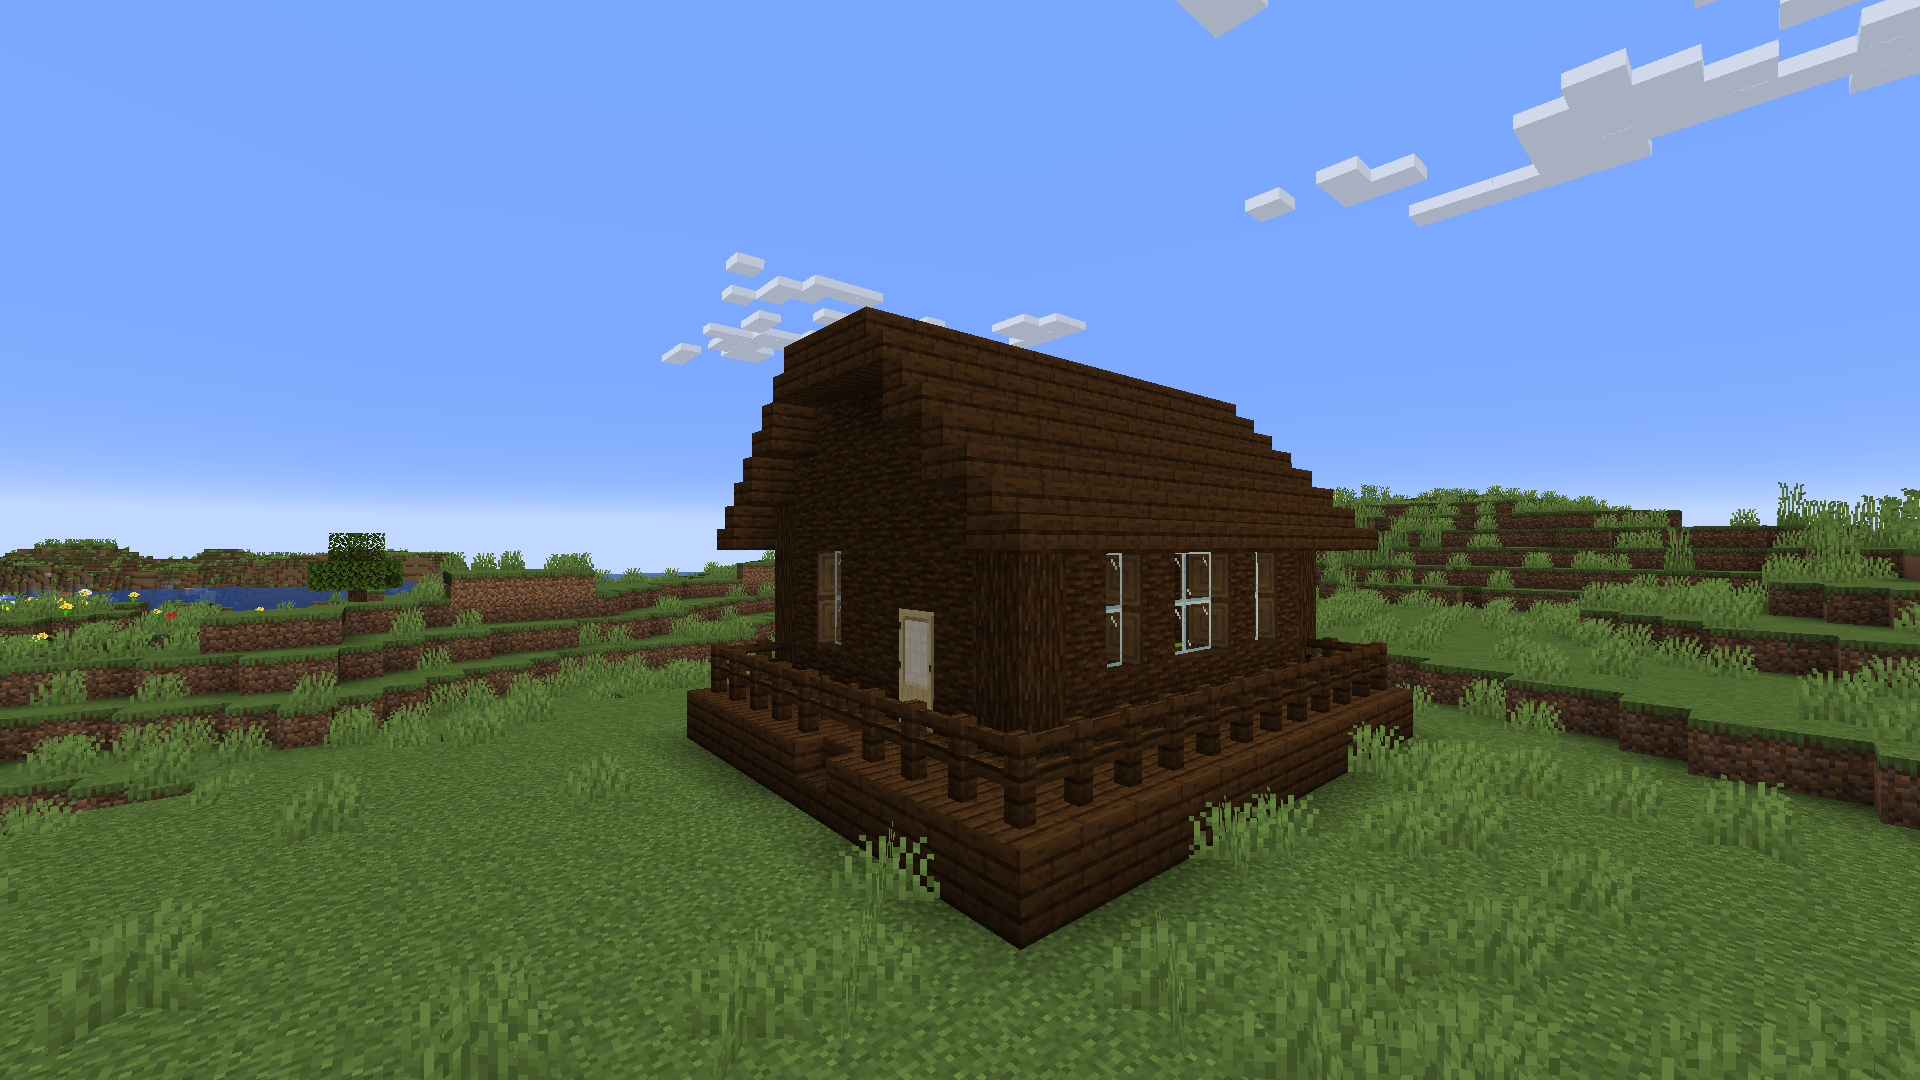
\includegraphics[width=0.5\textwidth]{../screenshots/plains.png}
    \centering
    \caption{Plains}
    \label{fig:plains}
\end{figure}
\begin{figure}
    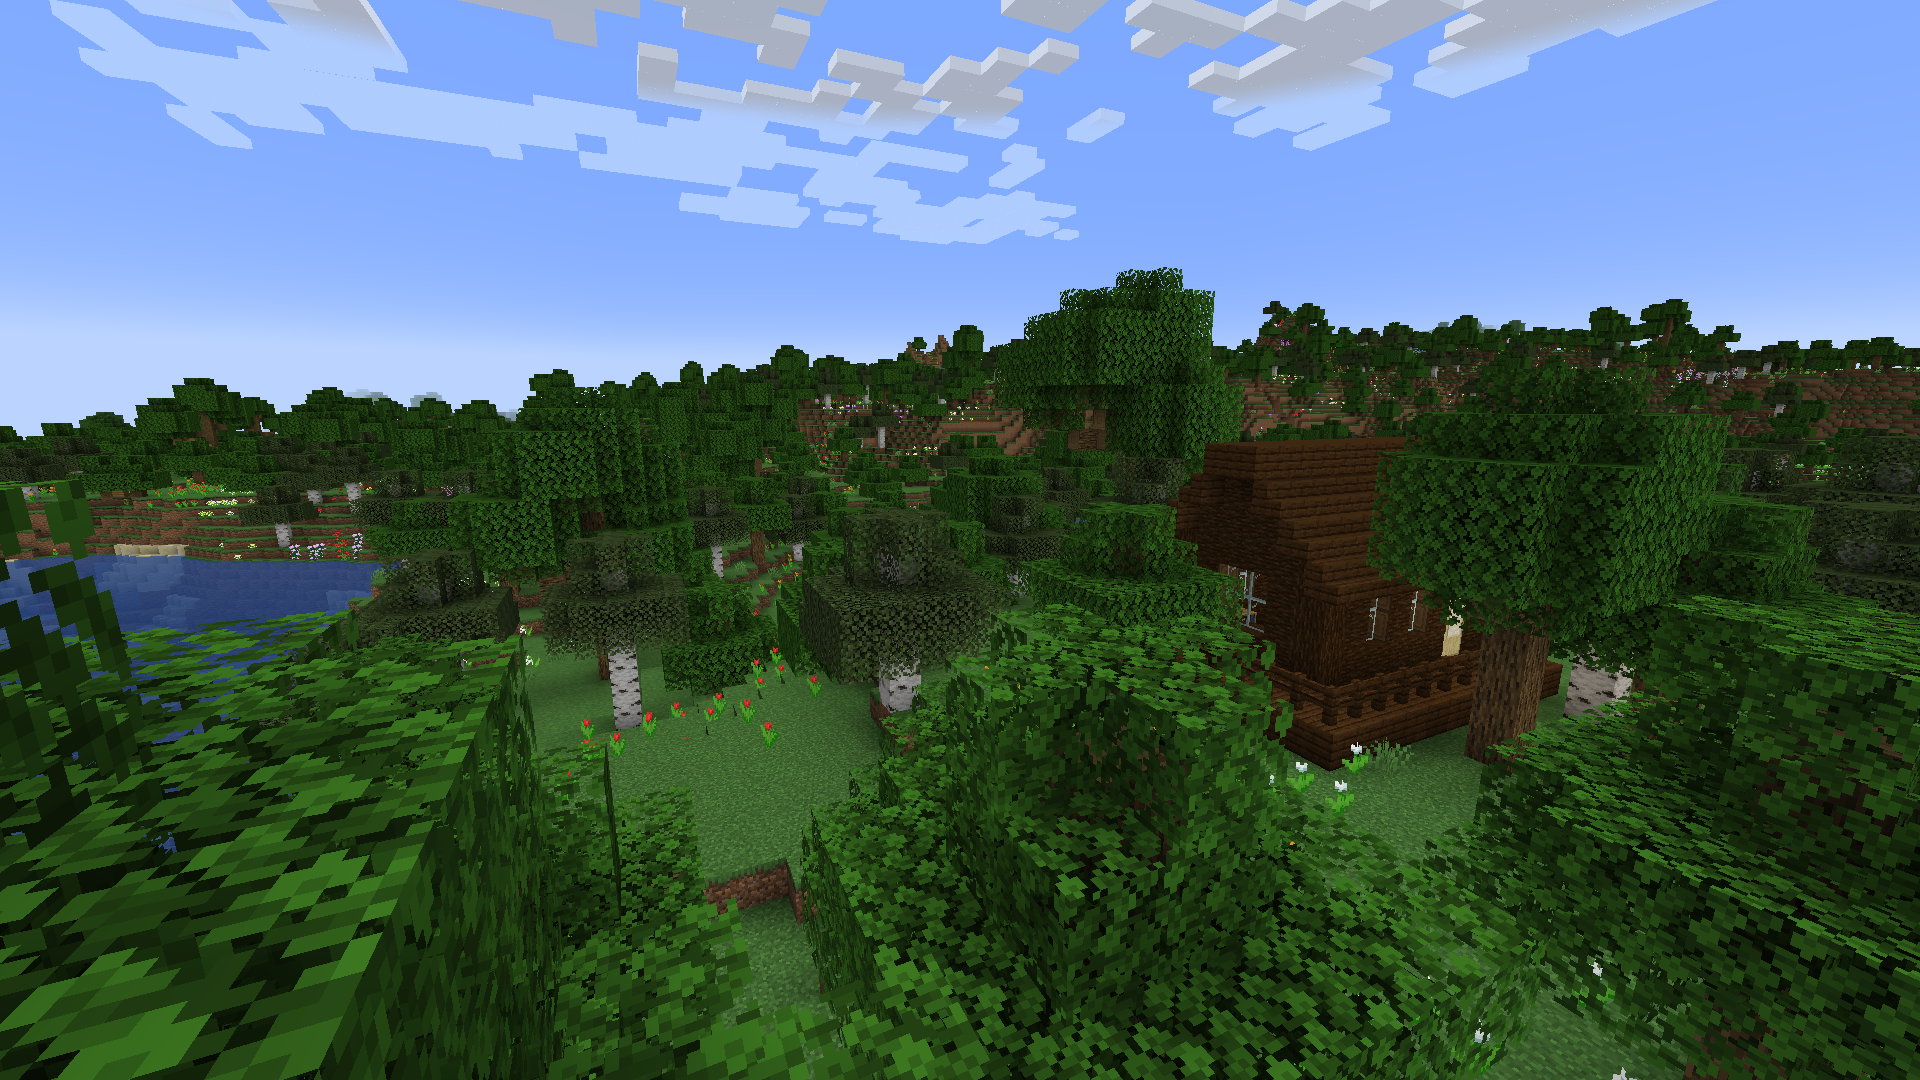
\includegraphics[width=0.5\textwidth]{../screenshots/forest.png}
    \centering
	\caption{(Flower) forest}
    \label{fig:forest}
\end{figure}
\begin{figure}
    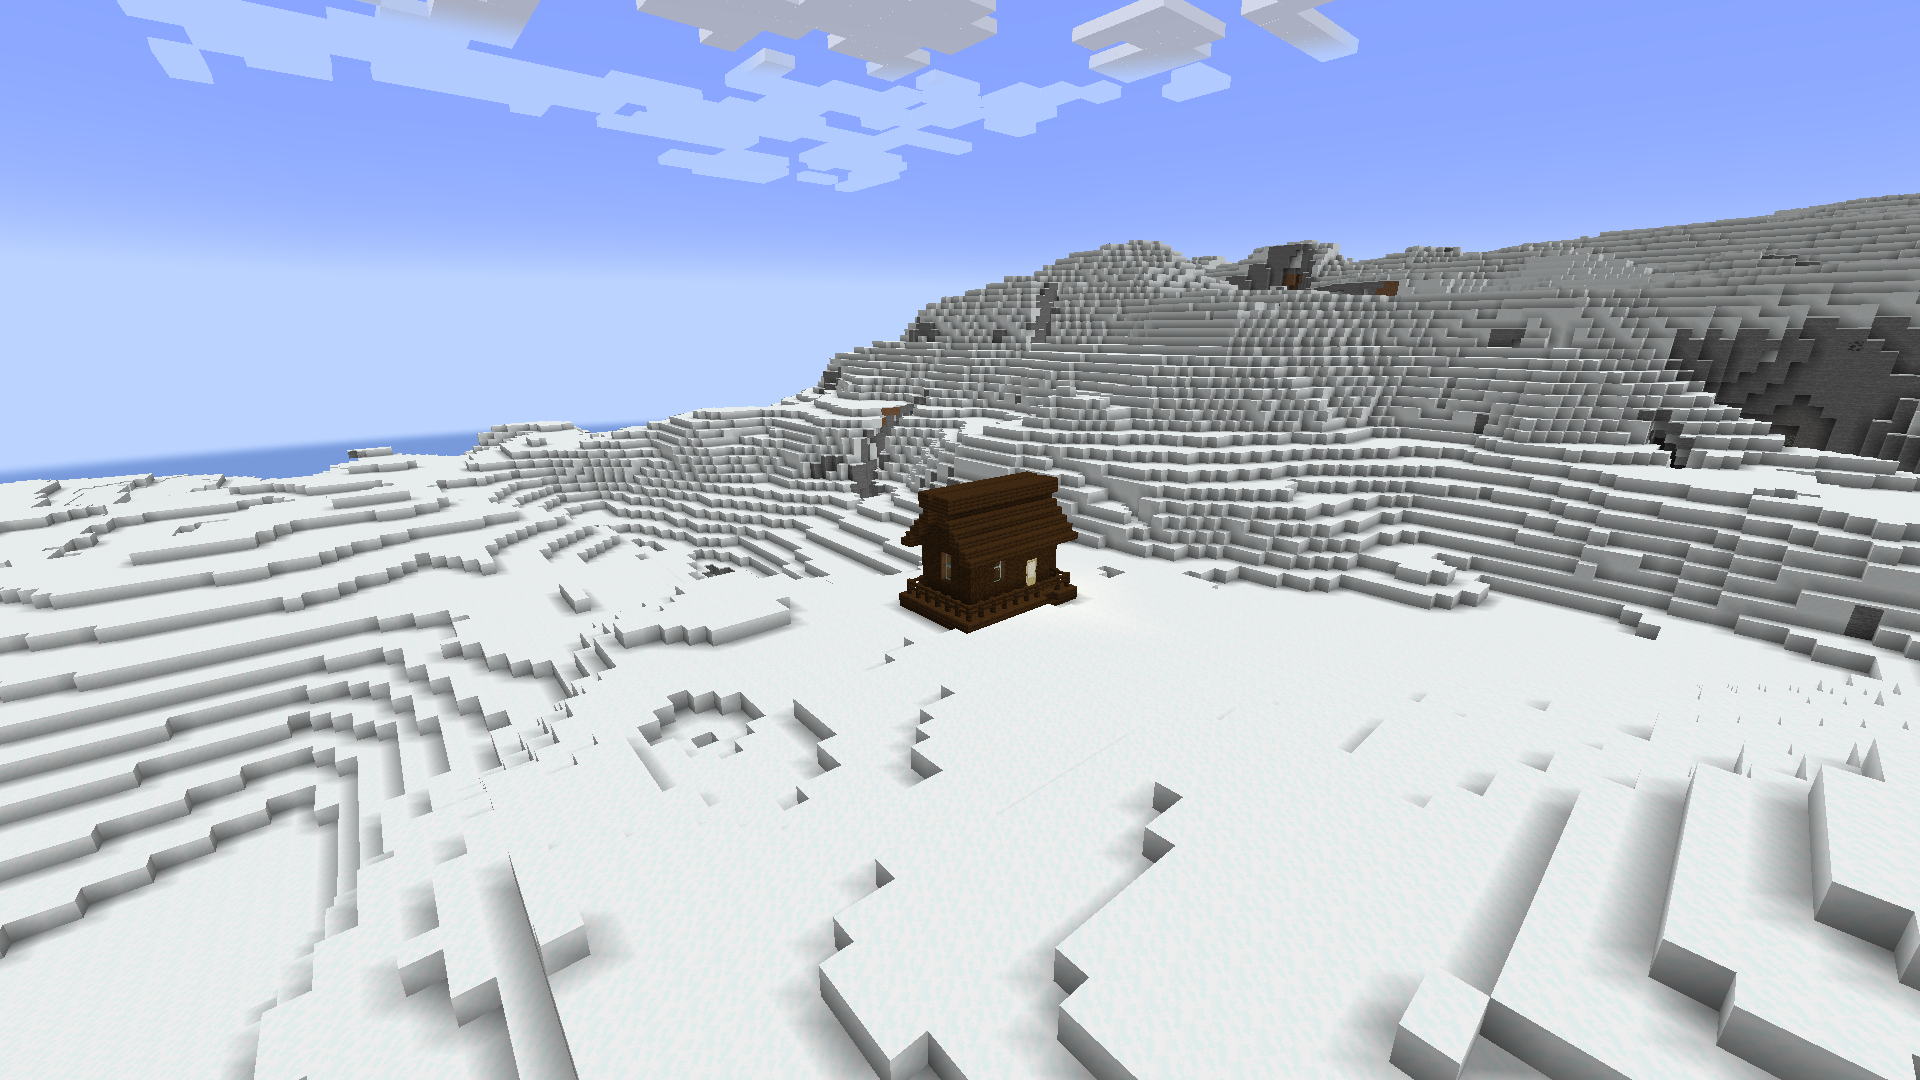
\includegraphics[width=0.5\textwidth]{../screenshots/hills.png}
    \centering
	\caption{(Snowy) hills}
    \label{fig:hills}
\end{figure}

Note window and door placement

\subsection{Limitations}
Jungle doesn't work

\section{Conclusion}
Just varying size makes the process of building quite complicated already

\printbibliography

\end{document}
